\section{Parametric Study}\label{sec:results}

\subsection{Elastic Modulus Sensitivity}

The $n=2$ flexural mode frequency depends strongly on the wall elastic
modulus $E$.  Table~\ref{tab:E_sweep} shows the predicted frequency for
a free shell across the physiologically relevant range.  The sweep
\SIrange{0.05}{2.0}{\mega\pascal} spans reported values from passive
peritoneum and relaxed abdominal wall tissue to tensed abdominal musculature
\cite{Deeken2017,Spadoni2024,Sack2023,parker2011imaging}.

\begin{table}[htbp]
  \centering
  \caption{Flexural mode $n=2$ frequency vs.\ elastic modulus
  ($a = \SI{0.18}{\metre}$, $c = \SI{0.12}{\metre}$, $h = \SI{10}{\milli\metre}$,
  $\nu = 0.45$, $\rho_w = \SI{1100}{\kilogram\per\metre\cubed}$,
  $\rho_f = \SI{1020}{\kilogram\per\metre\cubed}$).  The range
  \SIrange{0.05}{2.0}{\mega\pascal} is intended to bracket passive to active
  abdominal-wall stiffness reported in the abdominal mechanics and elastography
  literature \cite{Deeken2017,Spadoni2024,Sack2023,parker2011imaging}.}
  \label{tab:E_sweep}
  \begin{tabular}{rcc}
    \hline
    $E$ (MPa) & $f_2$ (Hz) & In ISO~2631 range? \\
    \hline
    0.05 & 3.4 & Marginal \\
    0.10 & 4.0 & Yes \\
    0.20 & 4.9 & Yes \\
    0.50 & 7.1 & Yes \\
    1.00 & 9.6 & Marginal \\
    2.00 & 13.3 & No \\
    \hline
  \end{tabular}
\end{table}

The \SIrange{4}{8}{\hertz} ISO~2631 abdominal resonance range requires
$E < \SI{0.5}{\mega\pascal}$, corresponding to relaxed, passive musculature.
Active muscle bracing increases $E$ by a factor of 10--100, moving the
resonance well above the infrasound range.  Figure~\ref{fig:freq_vs_E}
illustrates this dependence across the full physiological range.

\begin{figure}[htbp]
  \centering
  
\includegraphics[width=0.5\textwidth]{figures/fig_frequency_vs_E.pdf}
  \caption{Flexural mode frequencies vs.\ elastic modulus for modes
  $n = 2, 3, 4$.  The shaded band marks the ISO~2631 abdominal resonance
  range (\SIrange{4}{8}{\hertz}).  Relaxed musculature places the $n=2$ mode
  within this band; tensed muscle shifts it well above.}
  \label{fig:freq_vs_E}
\end{figure}

\subsection{Multi-Parameter Sensitivity}

A 486-point full factorial analysis varying $E$, $a$, $c/a$, $h$, and $\eta$
reveals that 37\% of configurations place the $n=2$ mode in the
\SIrange{5}{10}{\hertz} range and 41\% in the broader \SIrange{4}{8}{\hertz}
ISO~2631 range.  The separate Sobol sensitivity analysis below confirms that
$E$ dominates, followed by geometry and intra-abdominal pressure.

\subsection{Uncertainty Quantification}

A Monte Carlo simulation with $N = 10{,}000$ samples propagates parameter
uncertainties through the model.  Each parameter is drawn from a
physiologically motivated distribution: $E$ from a log-normal distribution
spanning \SIrange{0.05}{2.0}{\mega\pascal}, geometric parameters from normal
distributions matching anthropometric data, and the loss tangent from a
uniform distribution over $[0.10,\; 0.40]$.
A small number of Monte Carlo samples (25 of 10{,}000, or 0.25\%) drew
nonphysical negative wall thickness from the untruncated normal distribution
and were excluded; the reported statistics are computed from the remaining
9{,}975 samples.

The resulting distribution of $f_2$ has a median of \SI{6.4}{\hertz} with a
90\% credible interval of \SIrange{3.3}{15.5}{\hertz}
(Table~\ref{tab:uq_summary}).  This interval is deliberately conservative:
it reflects the simultaneous variation of \emph{all} model parameters across
their full physiological ranges and is therefore considerably wider than
any single-parameter sweep.  The canonical prediction $f_2 = \SI{3.95}{\hertz}$
lies within the credible interval but near its lower bound, corresponding to
the soft-tissue, relaxed-musculature baseline; the median is higher because
the log-normal modulus distribution samples stiffer configurations more
frequently.  The distribution is positively skewed,
reflecting the log-normal distribution of $E$.

\begin{table}[htbp]
  \centering
  \caption{Monte Carlo uncertainty quantification results ($N = 10{,}000$).
  Airborne displacement $\xi_\mathrm{air}$ and the ratio $\mathcal{R}_\mathrm{full}$ use the
  pressure-based airborne upper bound at \SI{120}{\decibel}; the
  energy-consistent airborne displacement is ${\sim}6.5\times$ smaller, so the
  corresponding ratio at fixed mechanical loading is ${\sim}6.5\times$ larger.}
  \label{tab:uq_summary}
  \begin{tabular}{lccc}
    \hline
    Quantity & Median & 90\% CI & Units \\
    \hline
    $f_2$ & 6.4 & [3.3, 15.5] & Hz \\
    $\xi_\mathrm{air}$ (120 dB, pressure-based upper bound) & 0.18 & [0.11, 0.39] & $\mu$m \\
    $\xi_\mathrm{mech}$ (0.5 m/s$^2$) & 1800 & [300, 8200] & $\mu$m \\
    $\mathcal{R}_\mathrm{full}$ (pressure-based airborne) & $10^4$ & [$2 \times 10^3$, $3 \times 10^4$] & --- \\
    SPL for PIEZO1/2 activation (pressure-based, 1\,$\mu$m)\footnote{The pressure-based displacement
      overestimates the true wall motion by a factor of ${\approx}\,6.5$
      because it neglects the extremely low radiation efficiency
      ($4\zeta_\mathrm{rad}\zeta_\mathrm{struct}/\zeta_\mathrm{total}^2 \sim 3 \times 10^{-14}$).
      Using the energy-consistent displacement
      (\S\ref{sec:coupling}), the PIEZO1/2 benchmark rises to
      ${\approx}\,\SI{151}{\decibel}$---a \SI{16}{\decibel} correction
      that represents the physically realisable SPL.}
      & 135 & [128, 139] & dB \\
    \hline
    \textbf{SPL for PIEZO1/2 activation (energy-consistent)} & $\mathbf{\approx\,151}$ & --- & dB \\
    \hline
  \end{tabular}
\end{table}

Sobol sensitivity analysis reveals that the elastic modulus accounts for
86\% of the total output variance (total-order index $S_T = 0.86$).
All other parameters contribute less than 10\% individually.  This result
has important experimental implications: any future verification effort should
prioritise \emph{in vivo} measurement of abdominal wall stiffness, as this
single parameter dominates the uncertainty budget (Figure~\ref{fig:sobol}).
Because Table~\ref{tab:uq_summary} uses the pressure-based airborne upper bound
and $a_\mathrm{rms} = \SI{0.5}{\metre\per\second\squared}$ for the mechanical
loading, its $\mathcal{R}_\mathrm{full}$ row should not be confused with the headline
energy-consistent SDOF upper bound of $3.3 \times 10^4$ quoted in
Section~\ref{sec:coupling}.

\begin{figure}[htbp]
  \centering
  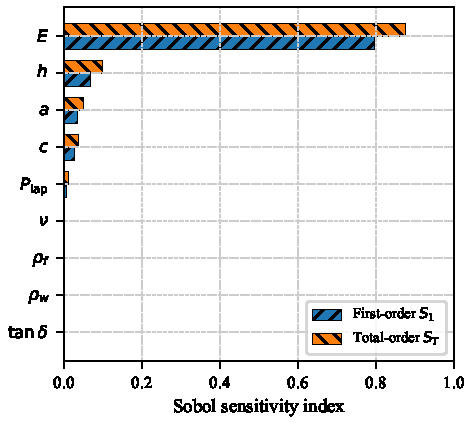
\includegraphics[width=0.5\textwidth]{figures/fig_uq_sobol_indices.pdf}
  \caption{Sobol first-order and total-order sensitivity indices for the $n=2$
  flexural frequency.  The elastic modulus $E$ accounts for 86\% of the total
  variance; all other parameters contribute less than 10\% individually.}
  \label{fig:sobol}
\end{figure}

\subsection{Multi-Layer Wall Model}

The abdominal wall comprises six distinct tissue layers:
peritoneum, transversalis fascia, internal oblique muscle, external oblique
muscle, subcutaneous fat, and skin.  Using classical laminate theory
\cite{Jones1999}, with layer thicknesses and relaxed/tensed tissue moduli
drawn from abdominal-wall measurements and soft-tissue elastography reviews
\cite{Deeken2017,Spadoni2024,Sack2023}, the effective composite modulus for a
relaxed wall is
$E_\mathrm{eff} \approx \SI{0.075}{\mega\pascal}$
($h_\mathrm{total} = \SI{25.1}{\milli\metre}$), giving
$f_2 = \SI{4.6}{\hertz}$---within approximately 16\% of the homogeneous model
prediction.
Muscle tension is confirmed as the dominant factor: tensed muscle
($E_\mathrm{eff} = \SI{2.7}{\mega\pascal}$) shifts $f_2$ to
\SI{23.1}{\hertz}.

\subsection{Boundary Condition Effects}
\label{sec:bc_effects}

The free-shell model in Section~\ref{sec:formulation} neglects the partial
constraints imposed by the spine, pelvis, and rib cage.  We quantify their
effect using a Rayleigh--Ritz analysis with Lamb-mode basis functions for
four progressively constrained configurations.
These configurations represent surrogate constraint cases chosen to bracket
the likely effect of anatomical boundary conditions, rather than a strict
monotonic continuation of a single geometry.

The Rayleigh--Ritz analysis employs a two-degree-of-freedom trial displacement
for each mode order $n$:
\begin{equation}
  w(\eta) = \beta\, P_n(\eta), \qquad
  u(\theta) = \alpha\, \sin\theta\, P_n'(\cos\theta),
\end{equation}
where $w$ is the normal (radial) displacement, $u$ is the tangential
(meridional) displacement, $P_n$ denotes the Legendre polynomial of degree
$n$, $\eta = \cos\theta$, and $\alpha$, $\beta$ are the Ritz coefficients
determined by minimising the Rayleigh quotient.  The basis functions are
chosen from the Lamb-mode family of free-sphere displacements; for partially
constrained configurations, the boundary conditions are enforced weakly through
the energy functional rather than strongly at discrete points.  In a strict
variational setting, such admissible trial functions provide upper bounds on
the natural frequencies; in the present reduced two-parameter implementation,
the free-shell Ritz frequency remains within 3\% of the closed-form Lamb value
(Table~\ref{tab:bc_results}).

Table~\ref{tab:bc_results} presents the results.  To assess the sensitivity of
the modal frequencies to boundary conditions, we performed a comparative
analysis using representative alternative parameters
($R = \SI{0.162}{\metre}$,
$\rho_f = \SI{1000}{\kilo\gram\per\metre\cubed}$,
$P_\mathrm{iap} = \SI{1500}{\pascal}$) chosen to match a specific mesh
geometry; these results are presented for relative comparison rather than
absolute prediction.  The free-sphere Ritz frequency ($f_2 = \SI{4.13}{\hertz}$) agrees
with the analytical prediction (\SI{4.26}{\hertz}) to within 3\%, providing a
useful numerical check.  The most constrained case---25\%
of the shell surface clamped---reduces $f_2$ by only \SI{11.4}{\percent}.  Even
the hemisphere-clamped case shifts the frequency by a mere \SI{5.8}{\percent}.

\begin{table}[htbp]
  \centering
  \caption{Rayleigh--Ritz Lamb-mode frequencies under various boundary
  conditions ($n=2$ flexural mode).}
  \label{tab:bc_results}
  \begin{tabular}{lcc}
    \toprule
    Configuration & $f_2$ (Hz) & Shift from free \\
    \midrule
    Free sphere (Ritz) & 4.13 & 0\% (verifies analytical) \\
    Hemisphere simply-supported & 3.91 & $-5.3\%$ \\
    Hemisphere clamped & 3.89 & $-5.8\%$ \\
    25\% surface clamped & 3.66 & $-11.4\%$ \\
    \bottomrule
  \end{tabular}
\end{table}

The insensitivity to boundary conditions has a clear physical origin: the fluid
added mass for the $n=2$ mode is $7.4\times$ the shell mass, so the system
inertia is dominated by the enclosed fluid rather than the wall.  In a dry
(empty) shell, the same boundary conditions would shift the frequency by
approximately \SI{33}{\percent}---but once the cavity is fluid-filled, the
added mass swamps the boundary stiffening effect.
Clamping part of the shell forces the incompressible fluid to redistribute
through a smaller aperture, increasing the effective modal mass.  When this
kinetic-energy increase exceeds the additional potential energy from the
constraint, the net effect is a frequency decrease.  We note that the 2-DOF
Ritz basis, which carries a ${\sim}\,9\%$ bias at the sphere limit, may also
contribute to this effect.
The \SI{6}{\percent} shift
is well within the $\pm 50$--$100\%$ uncertainty band set by material property
variability (\S\ref{sec:results}), confirming that the free-shell model is an
adequate approximation for the present purposes.

\subsection{Oblate Spheroid Correction}

The equivalent-sphere approximation used in Section~\ref{sec:formulation}
cannot capture the full geometric effect of an oblate shell.  To gauge the
size and sign of that effect, we also solved an exploratory Rayleigh--Ritz
model using oblate spheroidal basis functions, with proper account of the
spatially varying curvature and oblate fluid-mass geometry.  This comparison
must be interpreted cautiously: the same 2-DOF single-mode Ritz formulation
lies about \SI{9}{\percent} below the analytical sphere result even in the
sphere limit ($c/a \to 1$ for the canonical $n=2$ mode), owing to the
restricted trial-function space.  The 4--17\% differences in
Table~\ref{tab:oblate_correction} therefore should not be read as a precise
oblate correction.  Rather, they are exploratory and indicate the direction
and approximate magnitude of geometric effects: for the canonical oblate
shape, the more detailed model tends to reduce the flexural frequencies, with
the reduction becoming more pronounced at higher eccentricity and higher $E$,
where bending stiffness (which depends on local curvature) contributes a
greater share of the restoring force.

\begin{table}[htbp]
  \centering
  \caption{Illustrative equivalent-sphere vs.\ oblate spheroid Ritz frequencies for $c/a = 0.67$.}
  \label{tab:oblate_correction}
  \begin{tabular}{lcccc}
    \toprule
    & \multicolumn{2}{c}{$E = \SI{0.1}{\mega\pascal}$}
    & \multicolumn{2}{c}{$E = \SI{0.5}{\mega\pascal}$} \\
    \cmidrule(lr){2-3}\cmidrule(lr){4-5}
    Mode & Sphere (Hz) & Ritz (Hz) & Sphere (Hz) & Ritz (Hz) \\
    \midrule
    $n=2$ & 4.0 & 3.8 & 7.1 & 6.2 \\
    $n=3$ & 6.3 & 5.8 & 10.0 & 8.5 \\
    $n=4$ & 8.9 & 8.1 & 12.9 & 11.3 \\
    \bottomrule
  \end{tabular}
\end{table}

Taken indicatively, the exploratory oblate Ritz model moves the canonical
$n=2$ frequency from \SI{4.0}{\hertz} to approximately \SI{3.8}{\hertz}---still
within the ISO~2631 band and, if anything, closer to the low end of reported
abdominal resonance frequencies.

\subsection{Comparison with ISO~2631 Data}

Table~\ref{tab:iso} compares model predictions against published abdominal
resonance data.  This comparison serves as an independent consistency check: the model,
derived from first principles with no fitted parameters, predicts resonant
frequencies consistent with empirical whole-body vibration data compiled over
decades of occupational health research.  Agreement with ISO~2631 therefore
provides confidence that the shell model captures the essential physics of abdominal
resonance.

\begin{table}[htbp]
  \centering
  \caption{Model predictions vs.\ published abdominal resonance frequencies.}
  \label{tab:iso}
  \begin{tabular}{lcc}
    \hline
    Body type & $f_2$ (Hz) & ISO~2631 range? \\
    \hline
    Lean ($E = 0.2$, $a = 15$ cm) & 6.2 & Yes \\
    Average ($E = 0.1$, $a = 18$ cm) & 4.0 & Yes \\
    Large ($E = 0.08$, $a = 20$ cm) & 3.3 & Marginal \\
    \hline
  \end{tabular}
\end{table}
